\documentclass[12pt,a4paper,listof=totocnumbered]{scrartcl}
\usepackage{lscape}
\usepackage[ngerman]{babel}
\usepackage[utf8]{inputenc}
\usepackage{amsmath}
\usepackage{amsfonts}
\usepackage{amssymb}
\usepackage{graphicx}
\usepackage{fancyhdr}
\usepackage{tabularx}
\usepackage{geometry}
\usepackage{setspace}
\usepackage[right]{eurosym}
\usepackage[printonlyused]{acronym}
\usepackage{subfig}
\usepackage{floatflt}
%\usepackage{float}
\usepackage[usenames,dvipsnames]{color}
\usepackage{colortbl}
\usepackage{paralist}
\usepackage{array}
\usepackage{titlesec}
\usepackage{parskip}
\usepackage[right]{eurosym}
%\usepackage{picins}
\usepackage[subfigure,titles]{tocloft}
\usepackage[pdfpagelabels=true]{hyperref}
\usepackage{pdfpages} 
\usepackage{hyperref}
%\usepackage{minted}
\usepackage{listings}
\usepackage{fancyvrb}

\lstset{basicstyle=\footnotesize, captionpos=b, breaklines=true, showstringspaces=false, tabsize=2, frame=lines, numbers=left, numberstyle=\tiny, xleftmargin=2em, framexleftmargin=2em}
\makeatletter
\def\l@lstlisting#1#2{\@dottedtocline{1}{0em}{1em}{\hspace{1,5em} Listing #1}{#2}}
\makeatother

\DeclareNewTOC[%
 type=formel,
 name={Formel},%
 hang=5em,%
 listname={Formelverzeichnis}
]{for}

\newcommand*{\formelentry}[1]{%
 \addcontentsline{for}{formel}{\protect\numberline{Formel~\theequation} #1}%
}
\geometry{a4paper, top=25mm, left=25mm, right=25mm, bottom=35mm, headsep=10mm, footskip=12mm}


\hypersetup{unicode=true, pdftoolbar=true, pdfmenubar=true, pdffitwindow=false, pdfstartview={FitH},
	pdftitle={Projekt zur Lehrveranstaltung Data Warehousing},
	pdfauthor={Henry Glück, Paul Jaehne},
	pdfsubject={},
	pdfcreator={\LaTeX\ with package \flqq hyperref\frqq},
	pdfproducer={},
	pdfkeywords={},
	pdfnewwindow=true,
	colorlinks=true,linkcolor=black,citecolor=black,filecolor=magenta,urlcolor=black}

\begin{document}

\lstset{
  basicstyle=\ttfamily,
  columns=fullflexible,
  keepspaces=true,
  frame = none,
  aboveskip=10pt,
  belowskip=10pt
  }


\titlespacing{\section}{0pt}{12pt plus 4pt minus 2pt}{-6pt plus 2pt minus 2pt}

% Kopf- und Fusszeile
\renewcommand{\sectionmark}[1]{\markright{#1}}
\renewcommand{\leftmark}{\rightmark}
\pagestyle{fancy}
\lhead{}
\chead{}
\rhead{\thesection\space\contentsname}
\lfoot{}
\cfoot{}
\rfoot{\ \linebreak \thepage}
\renewcommand{\headrulewidth}{0.4pt}
\renewcommand{\footrulewidth}{0.4pt}

% Vorspann
\renewcommand{\thesection}{}
\renewcommand{\theHsection}{}
%\pagenumbering{Roman}

%----------------------------------------------------------------------------------------------------------
% Titelseite
%----------------------------------------------------------------------------------------------------------
\thispagestyle{empty}
\begin{center}
	
	\vspace*{2cm}
	\huge
	Hochschule für Technik, Wirtschaft und Kultur \\
	\vspace*{1cm}
	\large
	Fakultät Informatik, Mathematik und Naturwissenschaften\\
	
	
	\vspace*{2cm}
	\textbf{Projekt zur Lehrveranstaltung Data Warehousing}\\
	\vspace*{1cm}
	\large
	Betriebswirtschaftliche Analyse und Entwurf des Data Warehouse\\
	\vspace*{2cm}
	\textbf{Datum:} \today \\	
	\vspace*{2cm}
	\vfill
	\normalsize
	\newcolumntype{x}[1]{>{\raggedleft\arraybackslash\hspace{0pt}}p{#1}}
	\begin{tabular}{x{3.5cm}p{7.5cm}}
		\rule{0mm}{3ex}\textbf{Verfasser:} & Paul Jaehne und Henry Glück \\ 

	\end{tabular} 
\end{center}
\pagebreak


% ----------------------------------------------------------------------------------------------------------
% Verzeichnisse
% ----------------------------------------------------------------------------------------------------------
% TODO Typ vor Nummer

\setcounter{tocdepth}{2}

\renewcommand{\cfttabpresnum}{Tabelle }
\renewcommand{\cftfigpresnum}{Abbildung }
\settowidth{\cfttabnumwidth}{Abbildung 10\quad}
\settowidth{\cftfignumwidth}{Abbildung 10\quad}

\titlespacing{\section}{0pt}{12pt plus 4pt minus 2pt}{2pt plus 2pt minus 2pt}
\singlespacing

\rhead{INHALTSVERZEICHNIS}
\renewcommand{\contentsname}{Inhaltsverzeichnis}
\phantomsection
%\addcontentsline{toc}{section}{\texorpdfstring{\hspace{1.4em}Inhaltsverzeichnis}{Inhaltsverzeichnis}}
\addtocounter{section}{1}
\tableofcontents
\pagebreak
\rhead{VERZEICHNISSE}
\pagebreak

%--------------
% Abkürzungen
%\input{Abkuerzungen.tex}

\pagebreak



%----------------------------------------------------------------------------------------------------------
% Inhalt
%----------------------------------------------------------------------------------------------------------
% Abstände Überschrift
\titlespacing{\section}{0pt}{12pt plus 4pt minus 2pt}{-6pt plus 2pt minus 2pt}
\titlespacing{\subsection}{0pt}{12pt plus 4pt minus 2pt}{-6pt plus 2pt minus 2pt}
\titlespacing{\subsubsection}{0pt}{12pt plus 4pt minus 2pt}{-6pt plus 2pt minus 2pt}

% Kopfzeile
\renewcommand{\sectionmark}[1]{\markright{#1}}
\renewcommand{\subsectionmark}[1]{}
\renewcommand{\subsubsectionmark}[1]{}
\lhead{}
\rhead{\rightmark}

\onehalfspacing
\renewcommand{\thesection}{\arabic{section}}
\renewcommand{\theHsection}{\arabic{section}}
\setcounter{section}{0}
%\pagenumbering{arabic}
%\setcounter{page}{1}


%----------------------------------
% Phase1
%----------------------------------
\section{Betriebswirtschaftliche Analyse}
\subsection{Beschreibung möglicher Anwendungen aus Business-Sicht}
Zur betriebswirtschaftlichen Analyse sollen die Daten der Datenbank aus Sicht des Kundenmanagements, der Umsatzentwicklung und -verteilung, der Artikel- und Kategoriepflege sowie des Bestell- und Lieferprozesses allgemein betrachtet werden. Für diese Perspektiven wurden folgende folgende Fragestellungen festgelegt:  
\begin{itemize}
  \item Kundenmanagement:
  \begin{itemize}
    \item Wie viele Kunden hat der Shop ? 
    \item Wie ist die Altersverteilung der Kunden ?
    \item Wie hoch ist das Durchschnittsalter ?
    \item Wie oft bestellt der selbe Kunde bzw. Was ist die typische Zeitspanne zwischen zwei Bestellungen ?
    \item Wie hoch ist das Verhältnis zwischen Reklamationen und Bestellungen ?
    \item Was sind die Hauptgründe für Reklamationen ?
    \item Wer sind meine Top-Kunden ?
    \item Was sind die profitabelsten Altersgruppen ?  
  \end{itemize}
  \item Umsatzverteilung und -entwicklung:
  \item Artikel- und Kategoriepflege:
  \item Bestell- und Lieferprozesse:
\end{itemize}


Zur konzeptuellen Modellierung des Data Warehouse sowie zur Beantwortung der gestellten Fragen, wurden die folgenden Kennzahlen für die einzelnen Perspektiven definiert:
\begin{itemize}
  \item 
\end{itemize}

\subsection{Konzeptuelle Modellierung}
\subsection{Datenverarbeitungsanforderungen}


%----------------------------------
% Phase2
%----------------------------------
\section{Entwurf des Data Warehouse}
\subsection{Relationale Umsetzung eines MDM-Schemas}
Zur Realisierung, der in Phase 1 entworfenen Data Cubes, sollen die nachfolgenden relationalen Modelle verwendet werden. Es wurde sich hierbei für das Starflake-Schema entschieden, da es die Vorteile des Star- und Snowflake-Schemas vereint. Die notwendigen Befehle zum Anlegen der Dimensions- und Faktentabelle sind in der beigefügten SQL-Datei zu finden. 

\subsubsection{Data Cube für die Anzahl der Bestellungen}
\begin{figure}[htbp] 
    \centering
       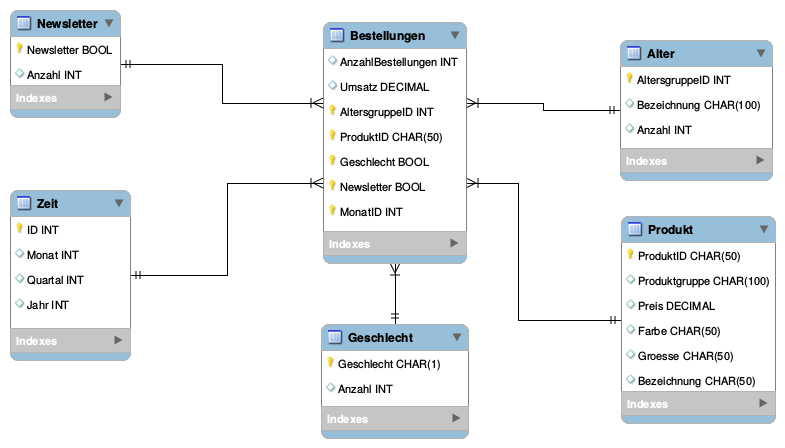
\includegraphics[width=0.8\textwidth]{phase2/dwh-bestellungen.png}
    \caption{Relationales Umsetzung des Cubes \glqq Bestellungen\grqq}
    \label{fig:bestellungen}
  \end{figure} 
   
Der Data Cube \glqq Bestellungen\grqq ~setzt sich aus der Faktentabelle \glqq Bestellungen\grqq ~und den Dimensiontabellen \glqq Alter\grqq ,~\glqq Produkt\grqq ~und \glqq Geschlecht\grqq ~zusammen. Die Dimension \glqq Zeit\grqq ~wurde gemäß dem Snowflake-Ansatz für eine bessere Datenintegrität in die Relationen \glqq Monat\grqq , \glqq Quartal\grqq ~und \glqq Jahr\grqq ~unterteilt.
\pagebreak

\subsubsection{Data Cube für die Anzahl der Retouren}
\begin{figure}[htbp] 
    \centering
       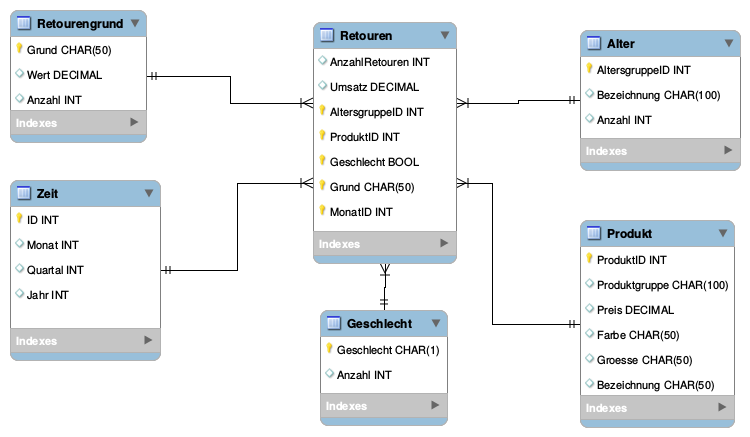
\includegraphics[width=0.8\textwidth]{phase2/dwh-retouren.png}
    \caption{Relationales Umsetzung des Cubes \glqq Retouren\grqq}
    \label{fig:retouren}
\end{figure}  
Analog zum Cube \glqq Bestellungen\grqq ~wurde auch der Data Cube \glqq Retouren\grqq ~zur Analyse der Reklamationen in eine Faktentabelle und mehrere Dimensionstabellen untergliedert. Auch hier wurde sich zur Verbesserung der Datenintegrität dazu entschieden, die Dimension \glqq Zeit\grqq ~in mehrere Tabellen aufzuteilen 
  
  
\subsubsection{Data Cube für Cross-Sells}
\begin{figure}[htbp] 
    \centering
       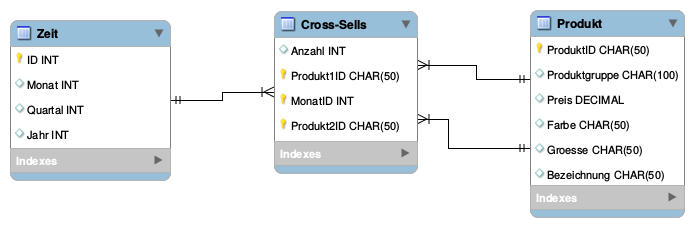
\includegraphics[width=0.72\textwidth]{phase2/dwh-cross.png}
    \caption{Relationales Umsetzung des Cubes \glqq Cross-Sells\grqq}
    \label{fig:bestellungen}
  \end{figure}  
  
Mithilfe des Data Cubes \glqq Cross-Sells\grqq ~soll, wie bereits erwähnt, untersucht werden, welche Produkte besonders häufig zusammen gekauft werden. Da zwischen den Produkten eine Art m-zu-n-Beziehung besteht, besitzt die Faktentabelle \glqq Cross-Sells\grqq ~zwei Fremdschlüssel auf die Dimensionstabelle \glqq Produkt\grqq . Auch bei diesem Cube wurde sich dazu entschieden, die zeitliche Dimension aufzuspalten.
  
\subsection{Optimierung der Data Cubes}
Zur Optimierung der Data Cubes stehen verschiedene Möglichkeiten zur Verfügung. So könnten durch materialisierte Sichten sowohl für die Cubes also auch für die Basis-Datenbank das Laden der Daten bzw. der Analyseprozess beschleunigt werden. Dabei wäre es ausreichend, wenn diese wöchentlich aktualisiert werden. Auch die Verwendung von Indexen wäre denkbar, um so die Abarbeitung bestimmter Analyseabfragen zu beschleunigen.









\end{document}
